\subsection{Preprocessing}
\label{subsec:prepro}
The proposed preprocessing steps for the T2-w MRIs consist of: bias correction using the N4ITK algorithm \cite{n4itk} followed by image intensity normalization to an interval of [0,1]. The region of interest (ROI), containing the prostate gland, was automatically subsampled as the intersection of the rectangular prisms of the three planes \cite{anneke}.The ROI is re-sampled to a resolution of $0.5 \times 0.5 \times 0.5$ mm  using linear interpolation \cite{itk}.Finally, after the images are cropped and resampled, they are linearly interpolated to an isotropic volume with resolution of $168^3$. Figure \ref{fig_1} shows an example of the resulting 2D slice of a T2-w MRI after being preprocessed with bias correction, normalization, cropped to a ROI, resampled, and interpolated to an isotropic volume. 



%\begin{figure}[h]
%    \centering
%    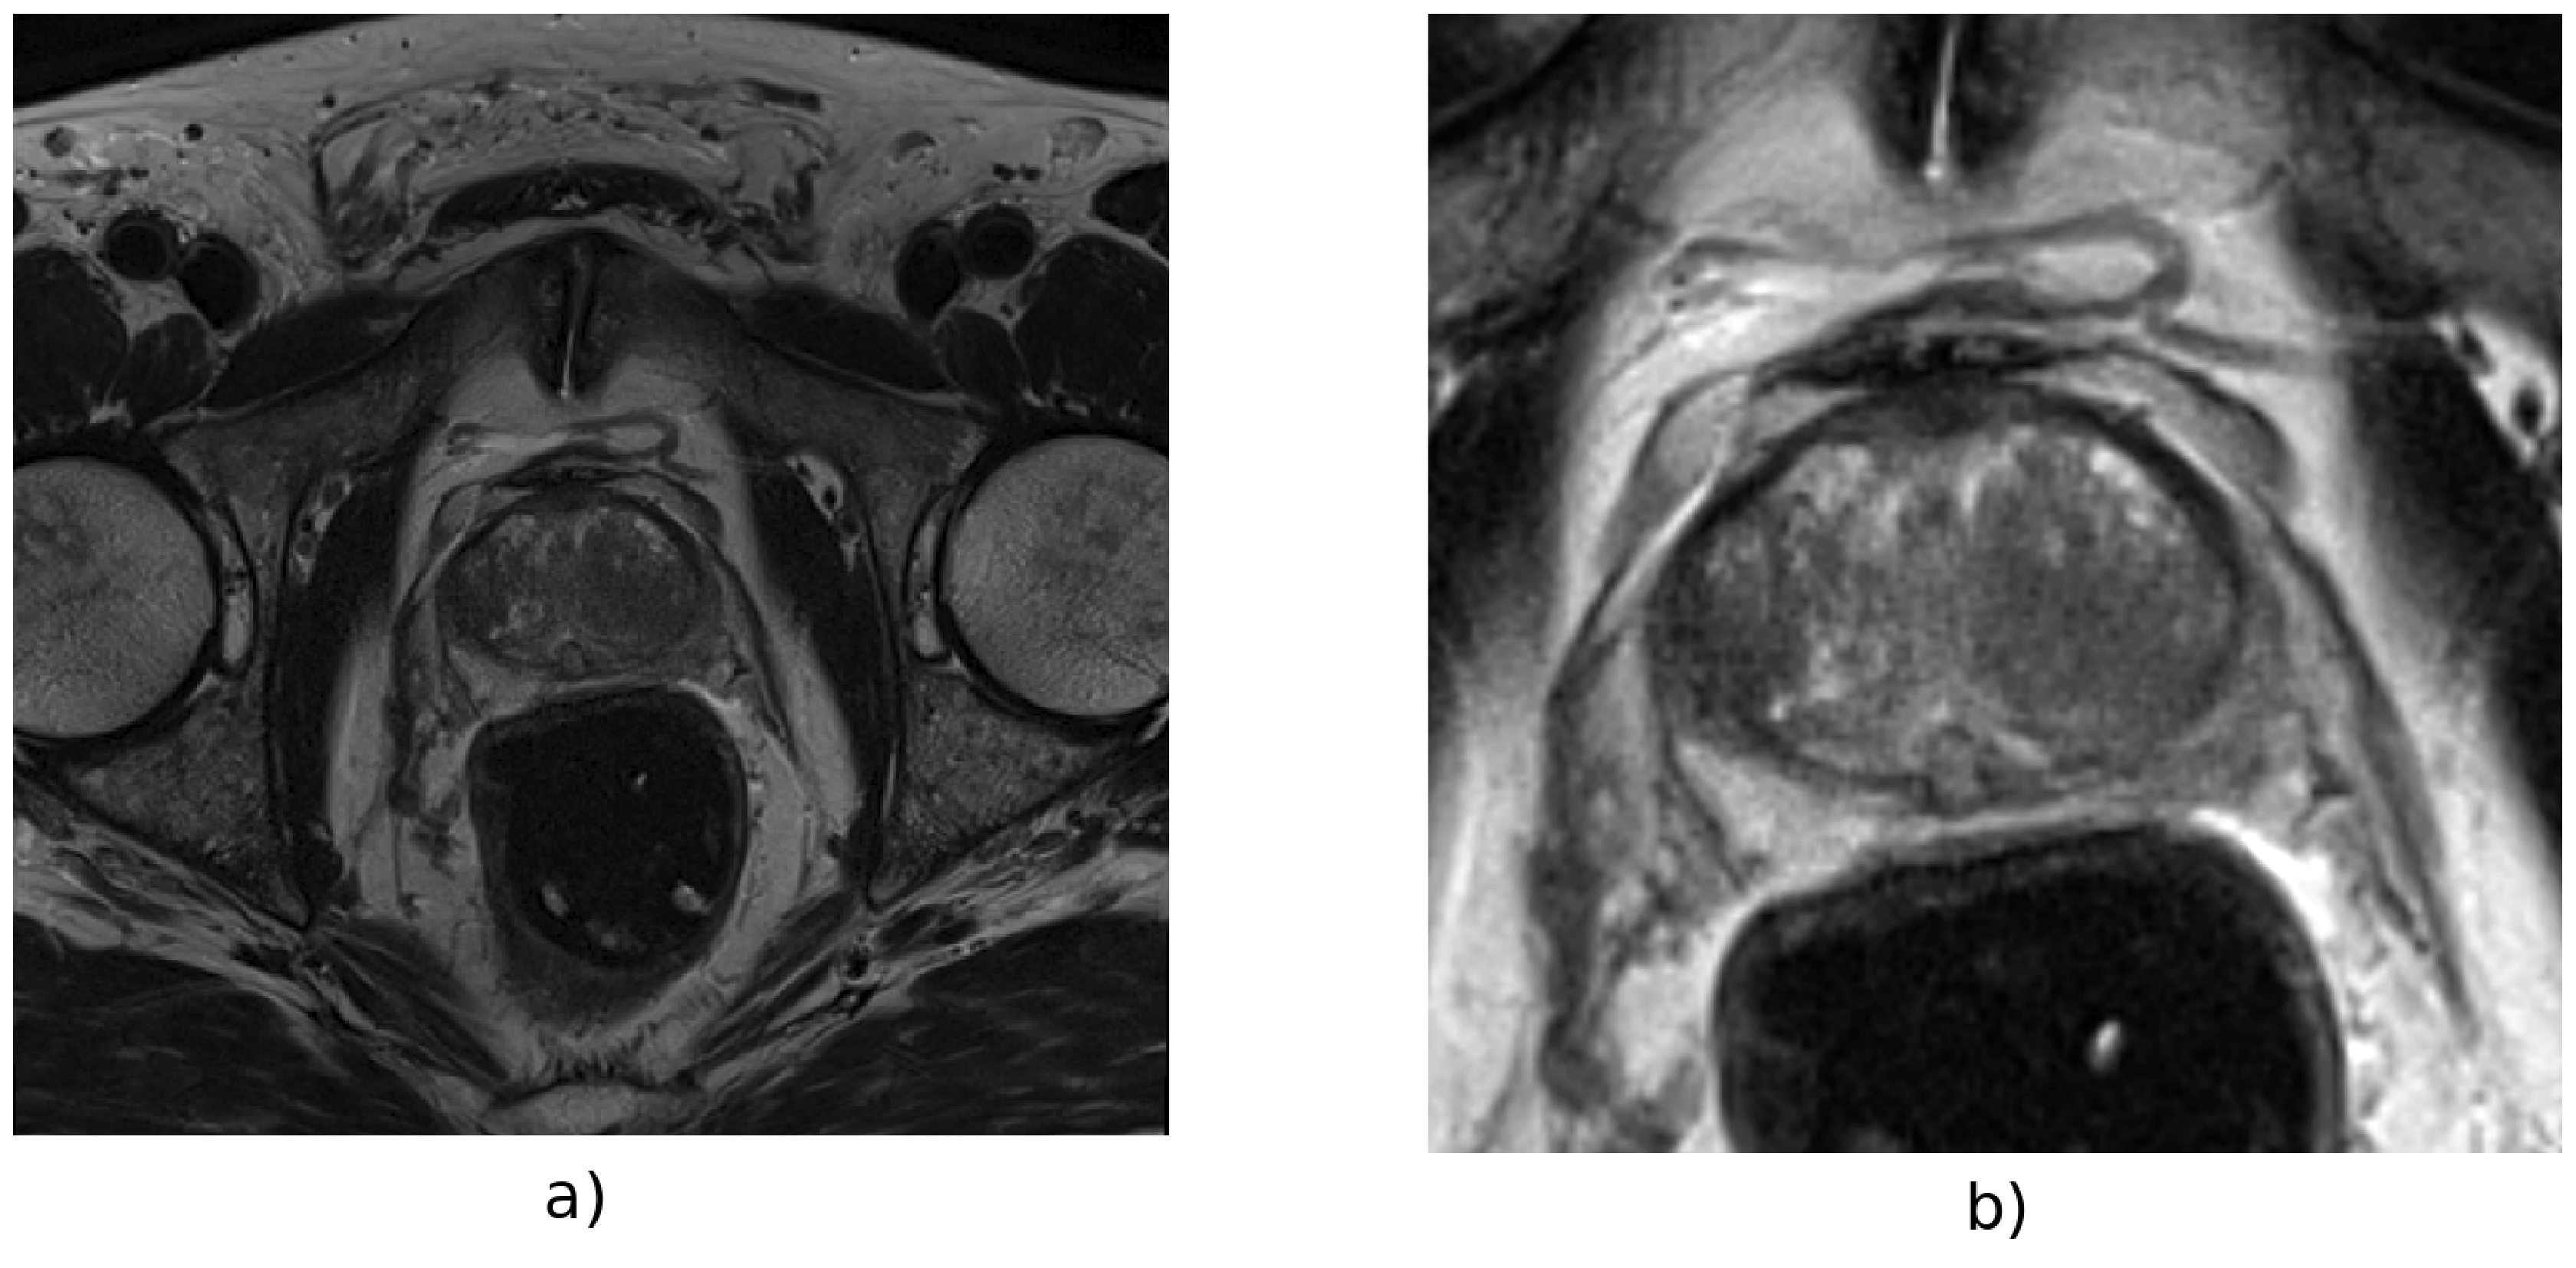
\includegraphics[totalheight=.25\textheight]{figures/Figure1.eps}
%    \caption{The MRIs are preprocessed with bias correction, normalization, resampling, and cropped to a ROI to reduce the variability of sizes and intensities between magnets. In this example, \textbf{a)} is the original image and \textbf{b)} is the image after being processed.} 
%    \label{fig_1}
%\end{figure}

Contour preprocessing included interpolation using optical flow.  The manual contours were carried out on the original T2-w MRI resolution and hence the necessity for interpolation. The proposed method focuses on obtaining intermediate contours between slices in the axial plane and is computed independently between every two consecutive horizontal slices. First, optical flow is obtained between the two contours of adjacent slices using the Farneback method \cite{optflow}. Then, intermediate contours are created by linear interpolation following the direction of the optical flow vector field. Figure \ref{fig:fig_2} shows an example of the optical flow obtained between two horizontal slices and the resulting interpolated 3D volume using this method. 

%\begin{figure}[h]
%    \centering
%    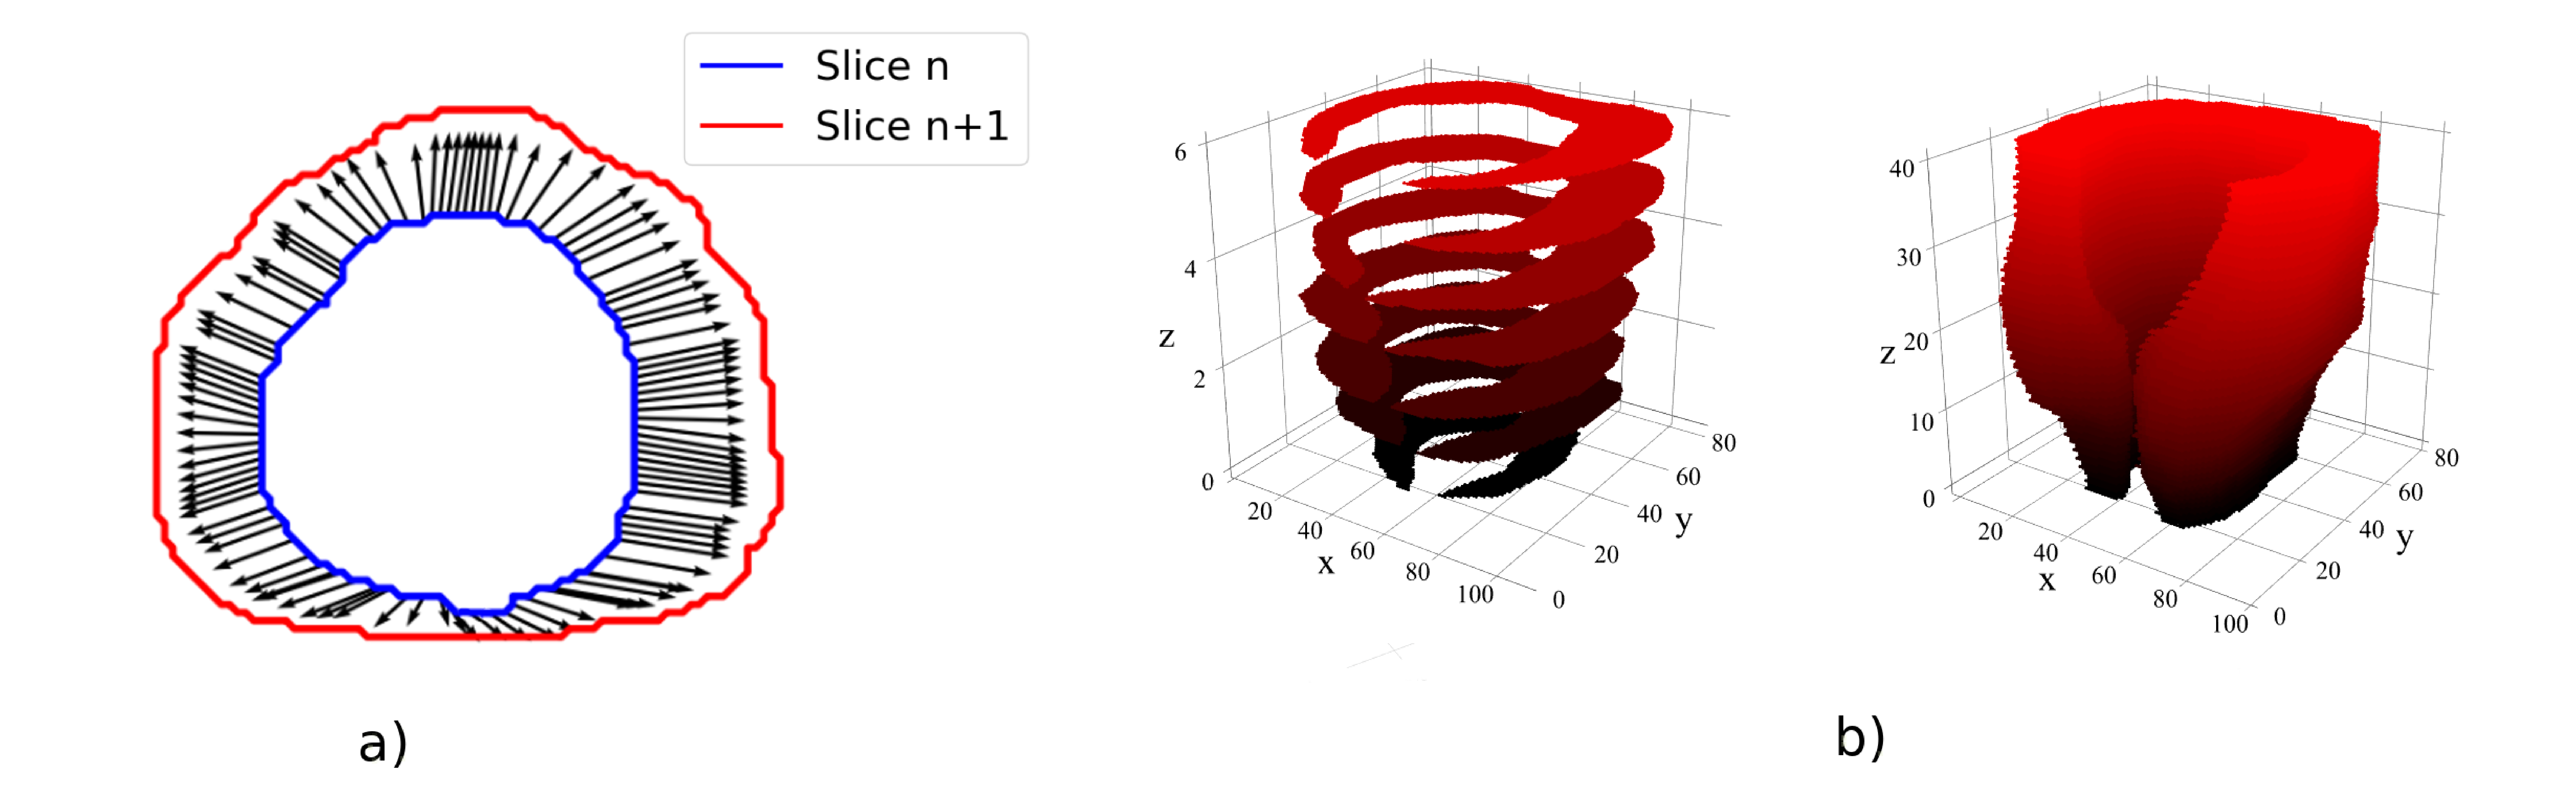
\includegraphics[totalheight=.21\textheight]{figures/Figure2.eps}
%    \caption{Example of the proposed algorithm to increase the resolution of prostate and PZ contours. In \textbf{a)}, an example of the optical flow obtained between two prostate contours from adjacent horizontal planes. In \textbf{b)} on the left, original contours with 17 slices. On the right, interpolated contours with 68 slices.}
%    \label{fig:fig_2}
%\end{figure}

